\documentclass[11pt,a4paper]{article}

% Packages
\usepackage[utf8]{inputenc}
\usepackage[T1]{fontenc}
\usepackage{geometry}
\usepackage{hyperref}
\usepackage{listings}
\usepackage{xcolor}
\usepackage{booktabs}
\usepackage{fancyhdr}
\usepackage{titlesec}
\usepackage{mdframed}
\usepackage{graphicx}
\usepackage{tikz}
\usetikzlibrary{shapes,arrows,positioning,calc}

% Page geometry
\geometry{margin=1in}

% Colors
\definecolor{codegreen}{rgb}{0,0.6,0}
\definecolor{codegray}{rgb}{0.5,0.5,0.5}
\definecolor{codepurple}{rgb}{0.58,0,0.82}
\definecolor{backcolour}{rgb}{0.97,0.97,0.95}
\definecolor{warningbg}{RGB}{255,243,205}
\definecolor{warningborder}{RGB}{255,234,167}
\definecolor{epoch0}{RGB}{70,130,180}    % Steel blue
\definecolor{epoch1}{RGB}{60,179,113}    % Medium sea green
\definecolor{epoch2}{RGB}{205,92,92}     % Indian red
\definecolor{epoch3}{RGB}{147,112,219}   % Medium purple

% Listings configuration
\lstdefinestyle{mystyle}{
    backgroundcolor=\color{backcolour},
    commentstyle=\color{codegreen},
    keywordstyle=\color{blue}\bfseries,
    numberstyle=\tiny\color{codegray},
    stringstyle=\color{codepurple},
    basicstyle=\ttfamily\small,
    breakatwhitespace=false,
    breaklines=true,
    captionpos=b,
    keepspaces=true,
    numbers=left,
    numbersep=5pt,
    showspaces=false,
    showstringspaces=false,
    showtabs=false,
    tabsize=4,
    frame=single,
    rulecolor=\color{black!30}
}
\lstset{style=mystyle}

% Header/Footer
\pagestyle{fancy}
\fancyhf{}
\fancyhead[L]{\texttt{Gantt Chart} Documentation}
\fancyhead[R]{\thepage}
\renewcommand{\headrulewidth}{0.4pt}

% Section formatting
\titleformat{\section}{\large\bfseries}{\thesection}{1em}{}
\titleformat{\subsection}{\normalsize\bfseries}{\thesubsection}{1em}{}

% Warning box
\newmdenv[
    linecolor=warningborder,
    backgroundcolor=warningbg,
    linewidth=1pt,
    roundcorner=3pt,
    innertopmargin=10pt,
    innerbottommargin=10pt,
    innerrightmargin=10pt,
    innerleftmargin=10pt
]{warningbox}

% Title
\title{\textbf{Gantt Chart Visualization Documentation}\\
\large Real-time Process Execution Timeline with PyQtGraph}
\author{}
\date{Updated: 2026-03-07}

\begin{document}

\maketitle
\thispagestyle{empty}

% AI Warning
\begin{warningbox}
\textbf{Warning:} This documentation was generated by an AI assistant. However I have reviewed this file and made changes accordingly if needed.
\end{warningbox}

\vspace{1em}

\begin{abstract}
\noindent The Gantt Chart module provides a comprehensive visualization of transformer training processes over time. It displays process execution timelines with task-based row grouping, epoch-colored bars, and synchronized crosshair interaction with resource monitoring plots. The implementation supports both manual and automatic refresh, epoch range filtering, and intelligent handling of parallel vs.\ sequential task execution.
\end{abstract}

\tableofcontents
\newpage

%==============================================================================
\section{Overview}
%==============================================================================

The Gantt Chart component is integrated into the \texttt{Training\_performance\_plotter.py} application as a toggleable panel in the Performance Reports tab. It visualizes process execution data from \texttt{eval\_results/processes.json} with the following key features:

\begin{itemize}
    \item \textbf{Task-Based Row Grouping}: Same tasks across different epochs share rows; parallel tasks get separate rows
    \item \textbf{Epoch-Colored Bars}: Different colors for different epochs with legend display
    \item \textbf{Time Synchronization}: Uses the same time reference as resource plots (earliest process init time)
    \item \textbf{Crosshair Sync}: Red vertical line on hover synchronizes with CPU/GPU/RAM plots
    \item \textbf{Epoch Range Filtering}: Respects selected epoch range from control panel
    \item \textbf{Refresh Functionality}: Manual refresh button and optional 5-second auto-refresh
    \item \textbf{Scrollable Labels}: Fixed label panel on the left that scrolls with the chart
\end{itemize}

%==============================================================================
\section{UI Layout}
%==============================================================================

The Gantt Chart panel uses a vertical splitter layout below the resource plots:

\begin{lstlisting}[language=Python, caption={Gantt Chart Container Layout}]
# Main container with controls
self.gantt_container = QtWidgets.QWidget()

# Top: Epoch legend
self.gantt_legend_layout = QtWidgets.QHBoxLayout()

# Middle: Scroll area with labels and chart
self.gantt_scroll_area = QtWidgets.QScrollArea()
self.gantt_content_widget = QtWidgets.QWidget()

# Bottom: Refresh controls
self.gantt_refresh_btn = QtWidgets.QPushButton("Refresh")
self.gantt_auto_refresh_checkbox = QtWidgets.QCheckBox("Auto")
self.gantt_status_label = QtWidgets.QLabel()
\end{lstlisting}

\subsection{Visual Layout Diagram}

Note: I have reviewed this section of the pdf, and I couldn't fix the diagram, but I am going to leave it as it is legible.

\begin{center}
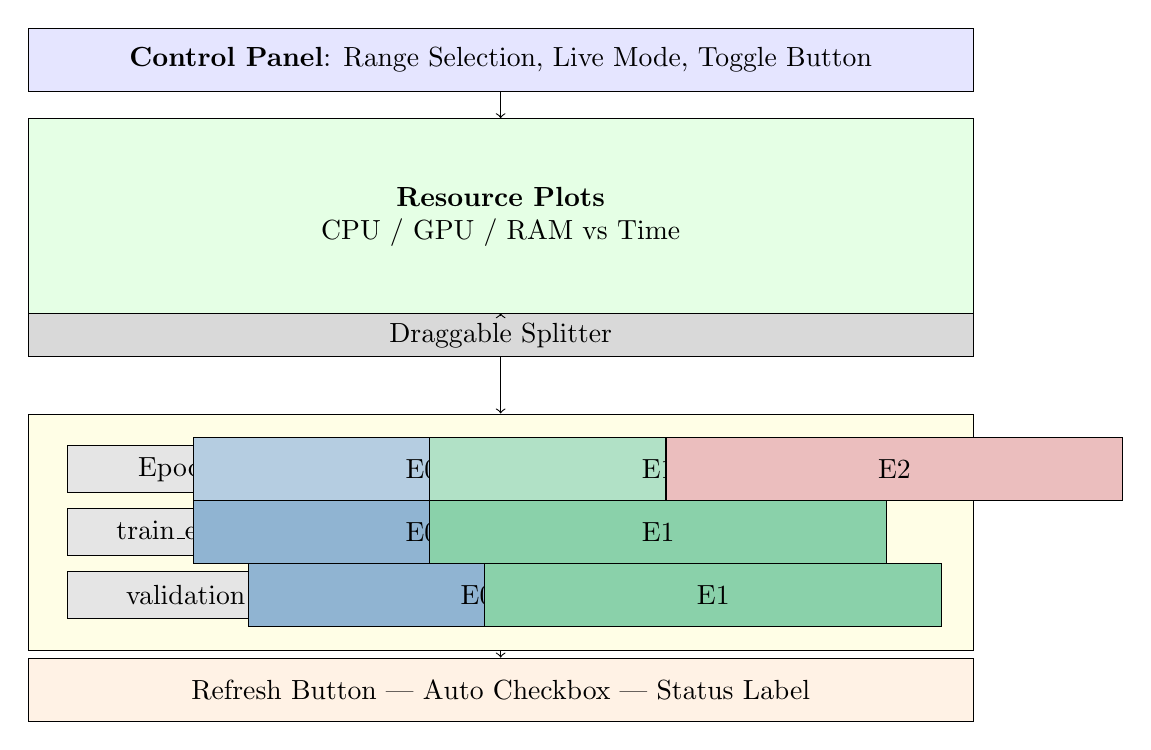
\begin{tikzpicture}[
    box/.style={draw, rectangle, minimum width=12cm, minimum height=0.8cm, align=center},
    smallbox/.style={draw, rectangle, minimum width=5.8cm, minimum height=0.8cm, align=center},
    label/.style={draw, rectangle, minimum width=3cm, minimum height=0.6cm, align=center, fill=gray!20}
]

% Control Panel
\node[box, fill=blue!10] (control) at (0,4) {\textbf{Control Panel}: Range Selection, Live Mode, Toggle Button};

% Resource Plots
\node[box, minimum height=2.5cm, fill=green!10] (plots) at (0,2) {\textbf{Resource Plots}\\CPU / GPU / RAM vs Time};

% Splitter
\node[box, minimum height=0.3cm, fill=gray!30] (splitter) at (0,0.5) {Draggable Splitter};

% Gantt Chart Area
\node[box, minimum height=3cm, fill=yellow!10] (gantt) at (0,-2) {};

% Gantt internals
\node[label] (epoch) at (-4,-1.2) {Epochs:};
\node[smallbox, fill=epoch0!40] (e0) at (-1,-1.2) {E0};
\node[smallbox, fill=epoch1!40] (e1) at (2,-1.2) {E1};
\node[smallbox, fill=epoch2!40] (e2) at (5,-1.2) {E2};

\node[label] (task1) at (-4,-2) {train\_epoch};
\node[smallbox, fill=epoch0!60] (t1) at (-1,-2) {E0};
\node[smallbox, fill=epoch1!60] (t2) at (2,-2) {E1};

\node[label] (task2) at (-4,-2.8) {validation};
\node[smallbox, fill=epoch0!60] (v1) at (-0.3,-2.8) {E0};
\node[smallbox, fill=epoch1!60] (v2) at (2.7,-2.8) {E1};

% Refresh controls
\node[box, fill=orange!10] (refresh) at (0,-4) {Refresh Button | Auto Checkbox | Status Label};

% Connections
\draw[->] (control) -- (plots);
\draw[->] (plots) -- (splitter);
\draw[->] (splitter) -- (gantt);
\draw[->] (gantt) -- (refresh);

\end{tikzpicture}
\end{center}

%==============================================================================
\section{Class Reference}
%==============================================================================

%------------------------------------------------------------------------------
\subsection{GanttChartWidget}
%------------------------------------------------------------------------------

The \texttt{GanttChartWidget} class extends \texttt{pg.GraphicsLayoutWidget} to provide the Gantt chart visualization.

\subsubsection{Constructor}

\begin{lstlisting}[language=Python]
class GanttChartWidget(pg.GraphicsLayoutWidget):
    """
    A Gantt chart widget for visualizing process execution timelines.
    
    Features:
    - Task-based row grouping (same task across epochs shares row)
    - Epoch-colored bars with labels
    - Crosshair synchronization with resource plots
    - Epoch range filtering support
    """
    
    def __init__(self, parent=None):
        super().__init__(parent)
        self.plot_item = self.addPlot(row=0, col=0)
        self.plot_item.setMenuEnabled(False)
        self.plot_item.setMouseEnabled(x=True, y=False)
        self.plot_item.hideButtons()
        self.crosshair_line = None
        self.processes_data = []
        self.base_time = 0
\end{lstlisting}

\subsubsection{Key Attributes}

\begin{table}[h]
\centering
\begin{tabular}{@{}llp{7cm}@{}}
\toprule
\textbf{Attribute} & \textbf{Type} & \textbf{Description} \\
\midrule
\texttt{plot\_item} & \texttt{PlotItem} & Main pyqtgraph plot for rendering bars \\
\texttt{crosshair\_line} & \texttt{InfiniteLine} & Red vertical line for time synchronization \\
\texttt{processes\_data} & \texttt{list} & Filtered process data for display \\
\texttt{base\_time} & \texttt{float} & Reference time (earliest process init) \\
\texttt{row\_assignments} & \texttt{dict} & Maps task names to row indices \\
\texttt{epoch\_colors} & \texttt{dict} & Maps epoch numbers to color values \\
\bottomrule
\end{tabular}
\end{table}

%------------------------------------------------------------------------------
\subsection{Task Grouping and Row Assignment}
%------------------------------------------------------------------------------

The Gantt Chart uses intelligent row assignment to handle both sequential and parallel processes:

\subsubsection{Base Task Name Extraction}

\begin{lstlisting}[language=Python]
def get_base_task_name(process_name: str) -> str:
    """
    Extract base task name by removing numeric suffixes.
    
    Examples:
    - 'train_epoch_05' -> 'train_epoch'
    - 'EncoderBlock_L0' -> 'EncoderBlock'
    - 'E5_B0042_SelfAttention' -> 'E5_B0042_SelfAttention'
    """
    # Remove trailing digits and underscores
    base_name = re.sub(r'_\d+$', '', process_name)
    return base_name or process_name
\end{lstlisting}

\subsubsection{Time-Aware Row Assignment}

\begin{lstlisting}[language=Python]
def assign_to_rows(processes: list) -> tuple:
    """
    Assign processes to rows based on task name and time overlap.
    
    Logic:
    1. Sort processes by start time
    2. For each process, find first row where it doesn't overlap
    3. Create new row if no suitable row exists
    
    Returns:
        (row_labels, row_processes): Labels for y-axis and 
                                      processes per row
    """
    # Sort by start time
    sorted_processes = sorted(processes, 
                              key=lambda p: p.get('start', 0))
    
    rows = []  # Each row is a list of (start, end, process)
    
    for proc in sorted_processes:
        base_name = get_base_task_name(proc['name'])
        start = proc.get('start', 0)
        end = proc.get('end', start)
        
        assigned = False
        for i, row in enumerate(rows):
            # Check for time overlap
            overlap = any(s < end and start < e 
                         for s, e, _ in row)
            if not overlap:
                rows[i].append((start, end, proc))
                assigned = True
                break
        
        if not assigned:
            rows.append([(start, end, proc)])
    
    # Generate labels with suffixes for parallel rows
    row_labels = []
    task_row_counts = {}
    for row in rows:
        if row:
            base_name = get_base_task_name(row[0][2]['name'])
            task_row_counts[base_name] = \
                task_row_counts.get(base_name, 0) + 1
    
    # ... create labels with (2), (3) suffixes for parallel rows
\end{lstlisting}

\textbf{Row Assignment Examples:}

\begin{table}[h]
\centering
\begin{tabular}{@{}lll@{}}
\toprule
\textbf{Processes} & \textbf{Result} & \textbf{Reason} \\
\midrule
Sequential train\_epoch\_00, \_01, \_02 & 1 row & No time overlap \\
Parallel EncoderBlocks & Multiple rows & Time conflict \\
LayerNorm in different epochs & 1 row & Sequential execution \\
\bottomrule
\end{tabular}
\end{table}

%------------------------------------------------------------------------------
\subsection{Data Loading}
%------------------------------------------------------------------------------

\subsubsection{Loading Process Data}

\begin{lstlisting}[language=Python]
def load_process_data(self, epoch_range=None):
    """
    Load process data from processes.json.
    
    Args:
        epoch_range: Optional tuple (start_epoch, end_epoch)
                     to filter processes
    """
    processes_file = Path("eval_results/processes.json")
    
    if not processes_file.exists():
        return
    
    with open(processes_file, 'r') as f:
        data = json.load(f)
    
    all_processes = []
    for uid, proc_data in data.get('processes', {}).items():
        epoch = Process.get_epoch_from_uid(uid)
        
        # Apply epoch range filter
        if epoch_range and epoch_range[0] is not None:
            if epoch < epoch_range[0] or epoch > epoch_range[1]:
                continue
        
        timeline = proc_data.get('timeline', {})
        init_time = timeline.get('initialized', 0)
        term_time = timeline.get('terminated', -1)
        
        if term_time < 0:
            term_time = init_time  # Ongoing process
        
        all_processes.append({
            'name': proc_data.get('name', 'Unknown'),
            'uid': uid,
            'epoch': epoch,
            'start': init_time,
            'end': term_time,
            'duration': term_time - init_time
        })
    
    self.processes_data = all_processes
    return self.processes_data
\end{lstlisting}

%------------------------------------------------------------------------------
\subsection{Rendering}
%------------------------------------------------------------------------------

\subsubsection{Rendering Gantt Bars}

\begin{lstlisting}[language=Python]
def render_gantt(self):
    """
    Render the Gantt chart with colored bars.
    
    Each bar represents a process execution:
    - X position: Start time (relative to base_time)
    - Width: Duration
    - Y position: Assigned row
    - Color: Based on epoch number
    - Label: Epoch identifier (E0, E1, etc.)
    """
    self.plot_item.clear()
    
    if not self.processes_data:
        return
    
    # Calculate base time from earliest process
    self.base_time = min(p['start'] for p in self.processes_data)
    
    # Assign rows using time-aware grouping
    row_labels, row_processes = assign_to_rows(self.processes_data)
    
    # Generate epoch colors
    unique_epochs = sorted(set(p['epoch'] 
                               for p in self.processes_data))
    self.epoch_colors = {}
    for i, epoch in enumerate(unique_epochs):
        self.epoch_colors[epoch] = pg.intColor(i, 
                                    len(unique_epochs))
    
    # Draw bars
    for row_idx, row in enumerate(row_processes):
        for start, end, proc in row:
            x = start - self.base_time
            width = end - start
            y = row_idx
            
            epoch = proc['epoch']
            color = self.epoch_colors[epoch]
            
            # Create bar item
            bar = pg.BarGraphItem(
                x=[x + width/2],
                y=[y],
                width=width,
                height=0.6,
                brush=color,
                pen=pg.mkPen(color='k', width=1)
            )
            self.plot_item.addItem(bar)
            
            # Add epoch label
            text = pg.TextItem(f"E{epoch}", anchor=(0.5, 0.5))
            text.setPos(x + width/2, y)
            self.plot_item.addItem(text)
    
    # Set Y axis labels
    self.plot_item.getAxis('left').setTicks(
        [(i, label) for i, label in enumerate(row_labels)]
    )
\end{lstlisting}

%==============================================================================
\section{Crosshair Synchronization}
%==============================================================================

The Gantt Chart crosshair synchronizes with the resource plots' vertical line:

\begin{lstlisting}[language=Python]
def set_crosshair_position(self, x_pos: float):
    """
    Set the crosshair line position.
    
    Called when hovering over resource plots to show
    corresponding time position in Gantt chart.
    
    Args:
        x_pos: X coordinate in seconds (relative to base_time)
    """
    if self.crosshair_line is None:
        self.crosshair_line = pg.InfiniteLine(
            angle=90,
            movable=False,
            pen=pg.mkPen(color='r', width=2, style=Qt.PenStyle.SolidLine)
        )
        self.plot_item.addItem(self.crosshair_line)
    
    self.crosshair_line.setValue(x_pos)
\end{lstlisting}

\subsection{Event Handling in Resource Plots}

\begin{lstlisting}[language=Python]
def _on_pReport_plot_hover(self, event):
    """
    Handle mouse hover on resource plots.
    
    Updates crosshair position in Gantt chart when hovering
    over CPU/GPU/RAM plots.
    """
    if not self.gantt_chart_visible:
        return
    
    # Get mouse position in plot coordinates
    mouse_point = self.cpu_plot.vb.mapSceneToView(event.scenePos())
    time_x = mouse_point.x()
    
    # Update Gantt chart crosshair
    self.gantt_chart.set_crosshair_position(time_x)
\end{lstlisting}

%==============================================================================
\section{Refresh Functionality}
%==============================================================================

\subsection{Manual Refresh}

\begin{lstlisting}[language=Python]
def _refresh_gantt_chart(self):
    """
    Manually refresh Gantt chart data.
    
    Reloads process data from JSON and re-renders the chart.
    Updates timestamp label to show last refresh time.
    """
    self._load_and_render_gantt()
    
    # Update status label
    current_time = datetime.now().strftime("%H:%M:%S")
    self.gantt_status_label.setText(f"Last updated: {current_time}")
\end{lstlisting}

\subsection{Auto-Refresh Timer}

\begin{lstlisting}[language=Python]
def _on_gantt_auto_refresh_changed(self, state):
    """
    Toggle auto-refresh timer.
    
    When enabled, refreshes the Gantt chart every 5 seconds.
    Useful for monitoring live training.
    
    Args:
        state: Qt.CheckState (Checked or Unchecked)
    """
    if state == Qt.CheckState.Checked:
        self.gantt_refresh_timer.start(5000)  # 5 seconds
    else:
        self.gantt_refresh_timer.stop()
\end{lstlisting}

%==============================================================================
\section{Time Synchronization}
%==============================================================================

To ensure the Gantt Chart aligns correctly with resource plots, both use the same time reference:

\begin{lstlisting}[language=Python]
def _get_process_min_time(self) -> float:
    """
    Get the earliest process initialization time from processes.json.
    
    This time serves as t=0 for both Gantt chart and resource plots,
    ensuring visual alignment between both views.
    
    Returns:
        Unix timestamp of earliest process, or None if no processes
    """
    processes_file = Path("eval_results/processes.json")
    
    if not processes_file.exists():
        return None
    
    with open(processes_file, 'r') as f:
        data = json.load(f)
    
    min_time = float('inf')
    for proc_data in data.get('processes', {}).values():
        timeline = proc_data.get('timeline', {})
        init_time = timeline.get('initialized', 0)
        if init_time > 0 and init_time < min_time:
            min_time = init_time
    
    return min_time if min_time != float('inf') else None
\end{lstlisting}

\subsection{Resource Plot Time Normalization}

\begin{lstlisting}[language=Python]
def update_pReport_plots(self):
    """
    Update resource plots with synchronized time reference.
    
    Uses process min time as t=0 to align with Gantt chart.
    """
    df = pd.read_csv(self.file_sec)
    
    # Normalize time using process min time
    process_min_time = self._get_process_min_time()
    if process_min_time is not None:
        df["time"] -= process_min_time
    else:
        df["time"] -= df["time"].iloc[0]  # Fallback
    
    # ... rest of plotting code
\end{lstlisting}

%==============================================================================
\section{Epoch Legend}
%==============================================================================

The epoch legend shows color mappings for each visible epoch:

\begin{lstlisting}[language=Python]
def _update_gantt_legend(self):
    """
    Update the epoch color legend above the Gantt chart.
    
    Creates colored checkboxes showing each epoch's color.
    Only shows epochs currently visible in the filtered range.
    """
    # Clear existing legend items
    while self.gantt_legend_layout.count():
        item = self.gantt_legend_layout.takeAt(0)
        if item.widget():
            item.widget().deleteLater()
    
    # Add label
    self.gantt_legend_layout.addWidget(
        QtWidgets.QLabel("Epochs:")
    )
    
    # Add epoch color boxes
    if hasattr(self.gantt_chart, 'epoch_colors'):
        for epoch, color in sorted(
            self.gantt_chart.epoch_colors.items()
        ):
            # Create colored checkbox
            checkbox = QtWidgets.QCheckBox(f"E{epoch}")
            checkbox.setChecked(True)
            
            # Set checkbox background color
            color_hex = color.name()
            checkbox.setStyleSheet(f"""
                QCheckBox {{
                    background-color: {color_hex};
                    padding: 2px 8px;
                    border-radius: 3px;
                }}
            """)
            
            self.gantt_legend_layout.addWidget(checkbox)
    
    # Add stretch to push everything left
    self.gantt_legend_layout.addStretch()
\end{lstlisting}

%==============================================================================
\section{Integration with Main Application}
%==============================================================================

\subsection{Toggle Visibility}

\begin{lstlisting}[language=Python]
def _toggle_gantt_chart(self):
    """
    Toggle Gantt chart visibility.
    
    Shows/hides the Gantt chart panel and adjusts the UI layout.
    Loads process data when first shown.
    """
    self.gantt_chart_visible = not self.gantt_chart_visible
    
    if self.gantt_chart_visible:
        self.gantt_container.show()
        self.gantt_toggle_btn.setText("Hide Gantt Chart")
        
        # Load data if not already loaded
        if not self.gantt_chart.processes_data:
            self._refresh_gantt_chart()
    else:
        self.gantt_container.hide()
        self.gantt_toggle_btn.setText("Show Gantt Chart")
\end{lstlisting}

\subsection{Splitter Configuration}

\begin{lstlisting}[language=Python]
# Create splitter between plots and Gantt
self.main_splitter = QtWidgets.QSplitter(
    Qt.Orientation.Vertical
)

# Add plots container (top)
self.main_splitter.addWidget(self.plots_container)

# Add Gantt container (bottom)
self.main_splitter.addWidget(self.gantt_container)

# Set initial sizes (70% plots, 30% Gantt)
self.main_splitter.setSizes([700, 300])

# Make both sections stretchable
self.main_splitter.setStretchFactor(0, 1)
self.main_splitter.setStretchFactor(1, 1)
\end{lstlisting}

%==============================================================================
\section{Usage Examples}
%==============================================================================

\subsection{Basic Usage}

\begin{enumerate}
    \item Start the Performance Plotter: \texttt{python Training\_performance\_plotter.py}
    \item Go to ``Performance Reports'' tab
    \item Click ``Show Gantt Chart'' button
    \item The Gantt chart loads process data from \texttt{eval\_results/processes.json}
\end{enumerate}

\subsection{Viewing Specific Epoch Range}

\begin{enumerate}
    \item Enter start and end epochs in the range fields
    \item Click ``Apply Range''
    \item Gantt chart updates to show only processes from selected epochs
\end{enumerate}

\subsection{Live Training Monitoring}

\begin{enumerate}
    \item Enable ``LIVE MODE'' checkbox
    \item Enable ``Auto'' checkbox in Gantt chart panel
    \item Gantt chart refreshes every 5 seconds during training
    \item New processes appear automatically as they complete
\end{enumerate}

\subsection{Synchronized Crosshair}

\begin{enumerate}
    \item Hover over CPU, GPU, or RAM plot
    \item Red vertical line appears at that time position
    \item Same line appears in Gantt chart at corresponding time
    \item See which processes were executing at that moment
\end{enumerate}

%==============================================================================
\section{File Locations}
%==============================================================================

\begin{table}[h]
\centering
\begin{tabular}{@{}lp{8cm}@{}}
\toprule
\textbf{File} & \textbf{Description} \\
\midrule
\texttt{eval\_results/processes.json} & Process execution data with timestamps \\
\texttt{Training\_performance\_plotter.py} & Main application with Gantt chart integration \\
\bottomrule
\end{tabular}
\end{table}

%==============================================================================
\section{Notes and Limitations}
%==============================================================================

\begin{itemize}
    \item \textbf{Data Source:} Requires \texttt{processes.json} to be generated by training script
    \item \textbf{Time Accuracy:} Uses process init/termination times; may not capture sub-process timing
    \item \textbf{Row Limit:} Large numbers of parallel tasks may require vertical scrolling
    \item \textbf{Auto-Refresh:} 5-second interval may cause flicker; use manual refresh for stable view
    \item \textbf{Memory Usage:} Large process files may slow down rendering; epoch filtering recommended
    \item \textbf{Crosshair Sync:} Only active when Gantt chart is visible
\end{itemize}

\end{document}
